\section{Introduzione}
\textit{VPN} è l'acronimo di \textit{Virtual Private Network}, ed indica diverse
tecnologie e protocolli utilizzati per connettere tra loro
reti locali, singoli host
ad una rete, singoli host tra loro. In ogni caso i componenti della VPN si trovano
fisicamente in sedi diverse. Questa \textit{connessione} avviene a diversi livelli dello stack
ISO/OSI, principalmente al livello 2 od al livello 3.\\
Si possono realizzare diverse topologie:
\begin{description}
	\item[Remote Access]Si realizza questa configurazione quando si vuole un connettere
	uno o più host ad una rete. Un esempio classico è quello di dipendenti che connettono
	il proprio dispositivo (PC, tablet, smartphone, etc \ldots) alla rete aziendale
	quando non si trovano in sede, potendo così accedere alle risorse che normalmente
	avrebbero disponibili solo se si trovassero fisicamente nella sede dell'azienda.
	\item[LAN-to-LAN]A volte ci si riferisce a questa topologia anche come \textit{Intranet
	VPN}. In questo caso, si utilizza una VPN per connettere tra di loro due o più
	reti che sono geograficamente dislocate in posti diversi. E' molto utile per aziende
	che hanno più sedi sul territorio (anche in diversi stati), e che desiderano connettere
	tra di loro le reti di ciascuna sede.
	\item[Extranet VPN]Si tratta di un caso speciale di \textit{Intranet VPN}, e si realizza
	quando quando l'accesso ad una certa rete viene ristretto, ovvero è possibile accedere
	solo ad alcune sue parti mediante VPN.
\end{description}
Ma cosa significa davvero \textit{connettere tra di loro più reti}? La domanda sorge
spontanea, poiché una volta che due reti sono in Internet, in qualche modo
esse sono (indirettamente) connesse tra loro. In Internet, una normale rete privata
raggiunge solo le risorse che altre reti hanno rese disponbili su Internet,
siano esse dei server web o dei server mail.
Semplificando, si potrebbe dire che le varie reti accedono alle varie risorse delle
altre \textit{a livello di protocolli applicativi}.\\
Nel caso delle VPN, \textit{connettere tra di loro più reti a diversi livelli dello
	stack ISO/OSI (o TCP/IP)} significa realizzare un collegamento \textit{ad un livello
più basso di quello applicativo}. La maggior parte delle VPN realizza un collegamento
al livello 2 od al 3, e questo ha i seguenti effetti pratici sulle $n$ reti connesse
tra di loro in VPN:
\begin{itemize}
	\item livello 2: le reti si trovano all'interno di un unico spazio di indirizzi IP
	      (con stesso indirizzo di rete), ed è \textit{come se fossero separate da uno switch}.
	\item Livello 3: le diverse reti sono ciascune in uno spazio di indirizzamento separato,
	      ed è \textit{come se fossero separate da un router}.
\end{itemize}
Supponendo che vi siano due reti, $A$ e $B$, connesse tramite una VPN al livello 3,
un host della rete $A$ può accedere a \textit{tutte} le risorse della rete $B$,
non solo quelle che $B$ espone verso la rete Internet.


Si distinguono tre tipologie di VPN:
\begin{description}
	\item[Secure VPN]Una VPN realizzata utilizzando crittografia dei dati in transito
	tra i diversi host/reti coinvolte, \textit{secure} poiché l'utilizzo di algoritmi
	crittografici (ammesso che siano utilizzati correttamente) garantiscono che nessun
	attaccante che intercetti tale traffico sia in grado di decifrarlo o alterarlo in
	qualsiasi modo.
	\item[Trusted VPN]Sono fornite dagli ISP, i quali garantiscono che nessun'altro
	cliente sia sullo stesso circuito VPN, \textit{trusted} poiché ci si fida di
	questa garanzia, inoltre, non vengono fornite particolari proprietà di sicurezza
	mediante protocolli crittografici.
	\item[Hybrid VPN]Termine che indica una VPN composta da tratti \textit{Secure}
	e da tratti \textit{Trusted}.
\end{description}
Di seguito, ci si concentrerà esclsuivamente sulla prima tipologia, poiché essa è
quella di interesse per MoonCloud.


\section{Anatomia}
Nell'ambito delle VPN del primo tipo, un pricipio base su cui si fonda il loro
funzionamento è quello dell'\textit{incapsulamento}. Si tratta di un termine
ben noto nell'ambito dei protocolli di rete, che può essere sintetizzato come
di seguito. Siano $A, B$ due protocolli di rete, con $A$ che si trova ad un livello
più basso rispetto ad $B$ (quindi più vicino al \textit{fondo} della pila
protocollare). Entrambi i protocolli hanno un \textit{header} ed un
\textit{payload}.\\
Si dice che \textit{B incapsula A} quando il payload di $B$ è costituito dall'intero
pacchetto di $A$ (cioè header e payload di $A$), come mostrato in figura \ref{fig:tunnelling}.
E' importante notare che l'incapsulamento può essere ulteriormente generalizzato,
non è richiesto che $A$ sia di un livello più basso rispetto a $B$. Nello pila
di protocolli di rete, sia essa ISO/OSI o TCP/IP, l'incapsulamento è il modo di
procedere normale, per cui ad esempio un segmento TCP ha nel proprio payload
un intero pacchetto IP, il cui a sua volta ha come payload un intero frame Ethernet.


\begin{figure}
	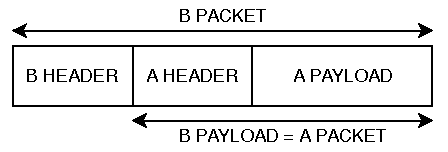
\includegraphics[scale=0.7]{img/tunnelling}
	\caption{Tunnelling}
	\label{fig:tunnelling}
\end{figure}


Di seguito si procede a dare una descrizione del funzionamento della maggior parte
delle VPN secure, iniziando con il definire con \textit{protocollo VPN}
il procollo utilizzato nel collegamento tra le reti/host.
Generalmente si distingue tra VPN client e VPN server, sebbene
una volta stabilito il collegamento il protocollo VPN sia spesso peer-to-peer
(nel senso che lo scambio di dati è bidirezionale);
in ogni caso vi è sempre un host che inizia la connessione.\\
Il VPN server può ricevere più connessioni dai VPN client, i quali in quanto tali
iniziano la connessione verso il server. A seconda della topologia/tecnologia,
i client possono essere responsabili di connettere alla rete del server la rete
a cui essi appartengono; viceversa, il server \textit{può} rendere visibile ai client
la rete cui appartiene. Altrettanto opzionalmente,
il server può connettere tra di loro i diversi client e le loro reti (nel senso che
i client possono comunicare tra loro anziché solo con il server/con la rete del server).\\
Per poter effettivamente collegare tra loro più \textit{reti}, il VPN \textit{peer}
deve avere i seguenti \textit{punti di contatto}:
\begin{itemize}
	\item collegamento con l'altro peer, raggiungibile tramite la rete Internet;
	\item punto di ricezione da cui riceve pacchetti provenienti dagli host della
	      rete in cui esso si trova e diretti alla rete dell'altro peer;
	\item punto di invio al quale l'host invia i pacchetti provenienti dalla rete dietro
	      la VPN
	      e diretti ad host della propria.
\end{itemize}
Il collegamento di cui al primo punto si realizza spesso (ma non sempre) con un socket,
mentre gli ultimi due punti si realizzano con una \textit{scheda di rete virtuale}.\\
Nel collegamento lungo il socket, la tecnologia VPN definisce un protocollo (che ovviamente
garantisca proprità di sicurezza), può essere un protocollo già esistente come TLS,
oppure uno sviluppato ad hoc.\\
Una scheda di rete virtuale (o virtual NIC -- Network Interface Card) è una
scheda di rete che esiste nel kernel del sistema
operativo ma che non ha un corrispettivo fisico. Se ne può creare una al livello 2
od al livello 3 (utilizzando \texttt{TUN}, modulo del
kernel implementato in diversi sistemi operativi). Una scheda di rete
al livello 3 è dotata di un indirizzo IP proprio come ogni NIC reale.\\
Una scheda di rete virtuale è associata ad un software che compie operazioni su essa,
e, come per ogni scheda di rete, tali operazioni sono quelle di invio e ricezione.
\begin{description}
	\item[Inviare]Il software associato invia un pacchetto sulla NIC, l'effetto è che tale
	pacchetto viene \textit{ricevuto} dal kernel del sistema operativo e processato
	come un qualsiasi altro pacchetto, pertanto l'OS deciderà
	dove e come inviarlo, e se applicare ulteriori trasformazioni.
	\item[Ricevere]Il sistema operativo riceve un pacchetto che ha per indirizzo destinazione
	quello delle scheda di rete virtuale, l'OS quindi inoltra il pacchetto alla NIC
	virtuale in questione, l'effetto è che il software associato riceve i dati
	che il sistema operativo ha inoltrato. Il pacchetto che viene inoltrato alla NIC
	può essere benissimo un pacchetto inviato da un altro host, e che quindi è arrivato
	al sistema operativo mediante una scheda di rete reale (oppure un'altra virtuale).
\end{description}
A livello di processo associato alla NIC, \textit{inviare un dato alla NIC} significa
chiamare la funzione \texttt{write()}, mentre \textit{ricevere} significa
utilizzare \texttt{read()} (o funzioni equivalenti).


L'idea di base è che ciò che il software VPN legge dalla scheda di rete virtuale
è ciò che è destinato ad un altro membro della VPN, e quindi venga incapsulato secondo
il protocollo VPN usato. Allo stesso modo, ciò che si riceve dal socket è destinato
alla proprio rete (salvo il caso si tratti di un server che connette più client), pertanto
viene scritto sulla NIC, per essere dato in gestione al proprio sistema operativo in
modo che possa inoltrarlo al destinatario.\\
Due note fondamentali che occorre sempre tenere presenti:
\begin{itemize}
	\item se si realizza una VPN al livello 3, tutte le reti partecipanti devono
	      avere degli spazi di indirizzamento diversi.
	\item In una VPN al livello 2, tutte le reti partecipanti devono stare
	      nella stessa rete IP.
\end{itemize}

Anche le schede di rete virtuali sono dotate di un indirizzo IP, in particolar modo
si definisce come \textit{subnet VPN} lo spazio di indirizzi dedicato alle NIC
che partecipano ad una stessa VPN. E' preferibile che tutte le NIC che compongono
una VPN abbiano lo stesso NET ID. A seconda delle tecnologie, il VPN server
può incorporare anche funzionalità di un DHCP server.


Per capire meglio quanto spiegato, si procede con un esempio.
Si supponga ora di voler configurare una certa \textit{VPN X}, e che si voglia realizzare una
topologia LAN-to-LAN tra due rete $A, B$, in cui nella prima si trova il server VPN $X$,
nella seconda naturalmente si trova il client.  Lo scenario è il seguente:
\begin{itemize}
	\item rete $A$: indirizzo di rete: \texttt{192.168.1.0/24}
	\item rete $B$: indirizzo di rete: \texttt{192.168.10.0/24}
	\item indirizzo interno del server VPN $s$ in $A$: \texttt{192.168.1.200}
	\item indirizzo pubblico del server VPN: \texttt{2.7.200.70}
	\item indirizzo interno del client VPN $c$ in $B$: \texttt{192.168.10.20}
\end{itemize}
Si definiscono
infine gli host \texttt{192.168.1.5} come $a_5$, e \texttt{192.168.10.5} in $b_5$, infine
si suppone che gli indirizzi IP
dei default gateway delle due reti finiscano in \texttt{.254}.\\
Per il momento non ci si concentra troppo sulla configurazione delle rotte, supponendo che i
pacchetti arrivino
agli host corretti. Si anticipa soltanto che in tutte le reti partecipanti alla VPN
(in questo caso $A$ e $B$), occorre configurare \textit{almeno una rotta}; nel capitolo in cui si descrivono le configurazioni di OpenVPN,
questo aspetto viene affrontato nel dettaglio.\\
Si vede quindi cosa succede quando $b_5$ vuole comunicare con $a_5$, posto che il
collegamento VPN tra $c$ ed $s$ sia già stato stabilito con successo. Si precisa che
si utilizza il termine generico \textit{pacchetto} per indicare un qualsiasi messaggio
di un qualsiasi protocollo di rete.
\begin{itemize}
	\item Il pacchetto da $b_5$ viene inviato, e quindi ricevuto da $c$.
	\item Il sistema operativo di $c$ invia il pacchetto alla scheda di rete virtuale
	      della VPN.
	\item Il pacchetto originale viene incapsulato da $c$ in un nuovo pacchetto secondo
	      il protocollo VPN, quindi inviato ad $s$ e da $s$ ricevuto.
	\item $s$ decifra (ed effettua verifiche di autenticità, integrità, ecc\ldots) il
	      pacchetto, a questo punto il risultato della decifratura è un pacchetto esattamente
	      uguale a quello generato al punto 1.
	\item $s$ scrive il pacchetto sulla propria scheda di rete virtuale.
	\item L'OS di $s$ riceve il pacchetto, lo invia a $a_5$.
\end{itemize}


Il protocollo di trasporto che viene in genere preferito è UDP in quanto introduce meno
overhead rispetto a TCP. A causa
dei particolari requisiti di MoonCloud, ci si è concentrati invece su soluzioni che
supportassero quest'ultimo, questo perché è possibile che nelle reti target UDP sia bloccato,
mentre è infattibile ritenere che TCP stesso sia bloccato (quanto meno si ritiene
che almeno il traffico HTTP sia consentito). Probabilmente vi saranno
delle restrizioni, e nel caso in cui la VPN non riesca a funzionare si può sempre
chiedere di aprire una porta sul firewall, l'importante è limitare il più possibile
questi casi.


\section{Topologie}
In questa sezione si esaminano le diverse topologie realizzabili per connettere una rete
target a MoonCloud. Non tutte le tecnologie VPN consentono di realizzare le topologie qui
dettagliate.
\begin{description}
	\item[\textit{LS - Local Server}]In questa configurazione si prevede di installare i
	VPN server in MoonCloud, mentre nelle reti target si porta il device
	VPN client, il quale è incaricato di connettersi al VPN server. Un server può essere
	potenzialmente responsabile per più reti client diverse, anzi questo
	è ciò che si vorrebbe. I container che fanno analisi
	(o l'host su cui sono in esecuzione)
	sono configurati per inoltrare i pacchetti al VPN server, il quale li invia alla rete
	target mediante il collegamento VPN.
	\item[\textit{RSMC - Remote Server Multi Client}]Opposta alla precedente, in \textit{RSMC}
	si installa un VPN server in ogni rete target. In una configurazione di tipo
	\textit{Multi Client}, ciascun Docker host è connesso direttamente in VPN con il server, il
	quale, una volta ricevuti i pacchetti dalla VPN li invia agli host target.
	\item[\textit{RSSC - Remote Server Single Client}]Simile ad \textit{RSMC}, il VPN
	server è presente nella rete target, in MoonCloud si realizza, per ciascuna rete
	target, un unico VPN client, a cui i Docker host responsabili per una certa rete target inviano
  i pacchetti. Quest'unico VPN client fungerebbe quindi da gateway per i target.
  Il client invia i pacchetti lungo la VPN al server,
	che provvede ad inoltrarli agli host nella rete target.
\end{description}
Nelle configurazioni di tipo \textit{Remote Server}, è necessario che il server sia
direttamente raggiungibile da MoonCloud, e quindi deve disporre di un indirizzo IP pubblico.
Si è supposto ragionevolmente che la rete target disponga di un collegamento ad Internet, e che
sia dietro router/firewall che esegua NAT. Poiché vi è NAT, è fondamentale che il server disponga
di un qualche meccanismo di NAT Traversal, poiché si vuole evitare di dover configurare
port forwarding sul router del cliente.\\
Vi sono naturalmente casi in cui non c'è NAT, ma sono una minoranza.\\
In configurazini \textit{Local Server} il problema non si pone perché la comunicazione viene
\textit{iniziata} dall'interno della rete target.

\begin{figure}[h]
	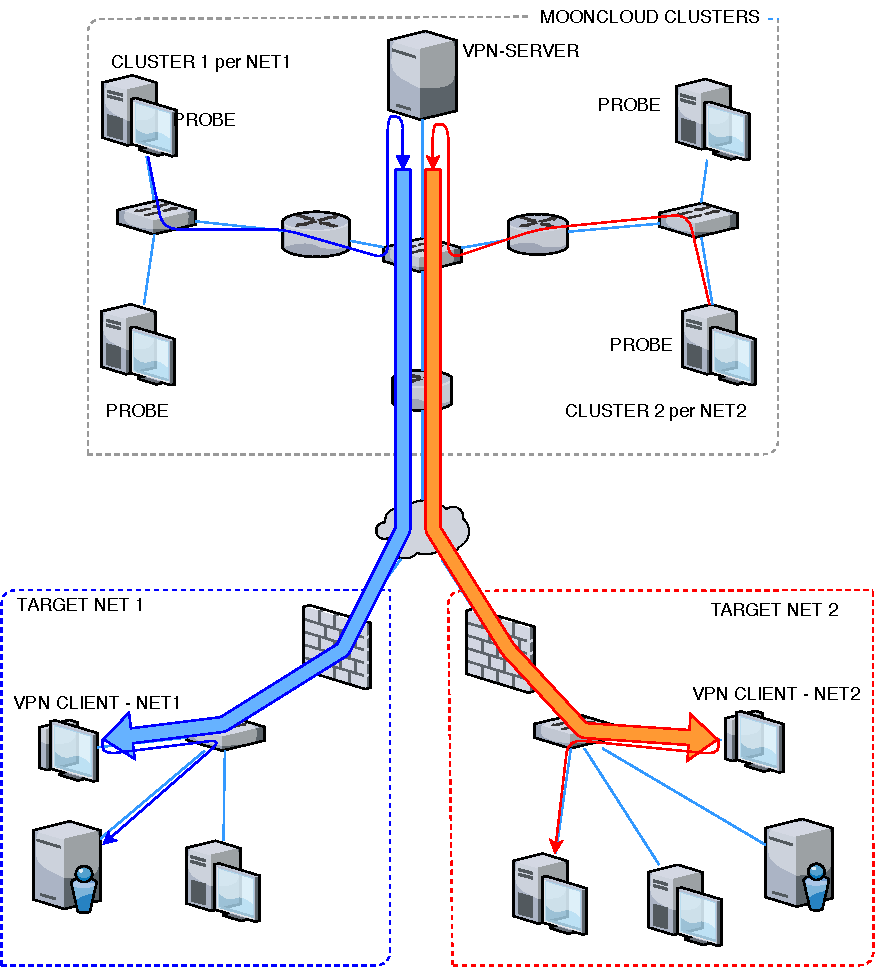
\includegraphics[scale=0.6]{img/ls}
	\label{fig:ls}
	\caption[Configurazione \textit{Local Server}]{Configurazione \textit{Local Server}. Le frecce
		più spesse mostrano il traffico che transita sulla VPN (di due colori diversi per identificare
		le due reti), mentre quelle \textit{thin} indicano del traffico non incapsulato.}
\end{figure}

\begin{figure}[h!]
	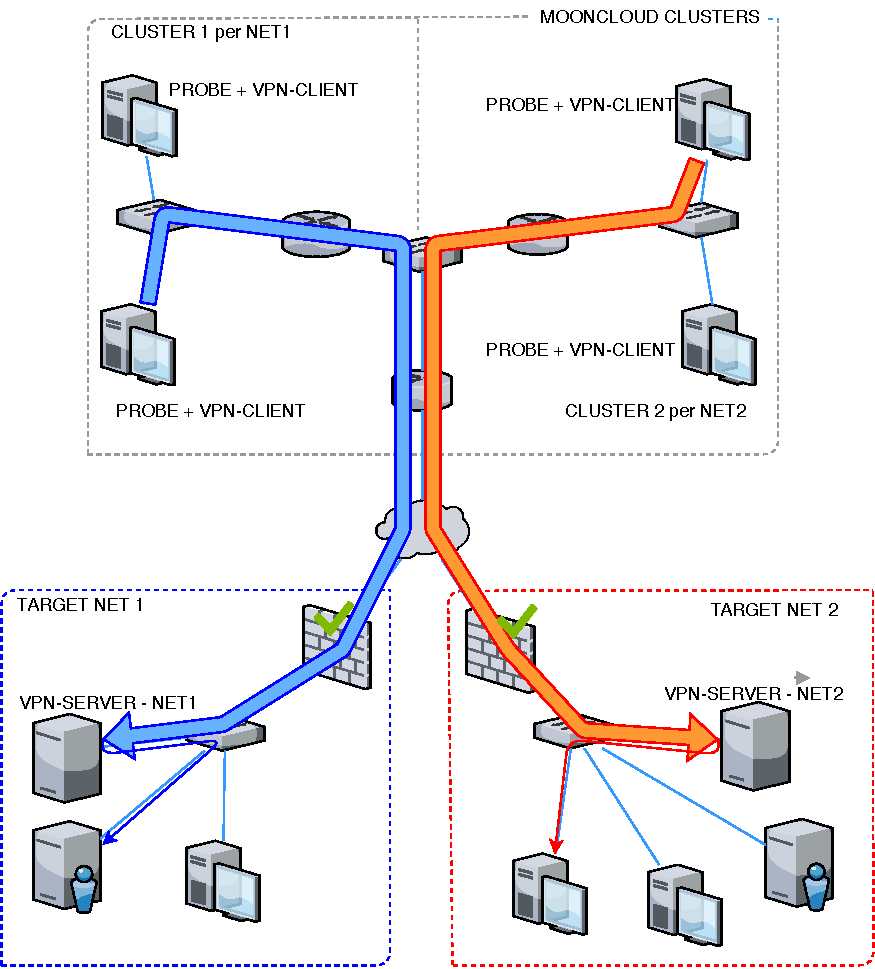
\includegraphics[scale=0.55]{img/rsmc}
	\label{fig:rsmc}
	\caption[Configurazione \textit{RSMC -- Remote Server Multi Client}]{Configurazione
		\textit{RSMC -- Remote Server Multi Client}. Ciascun probe è \textit{anche} un VPN client.
		La spunta verde sui firewall nelle reti target indica che deve essere consentito l'accesso
	dall'esterno verso i VPN server.}
\end{figure}

\begin{figure}[h!]
	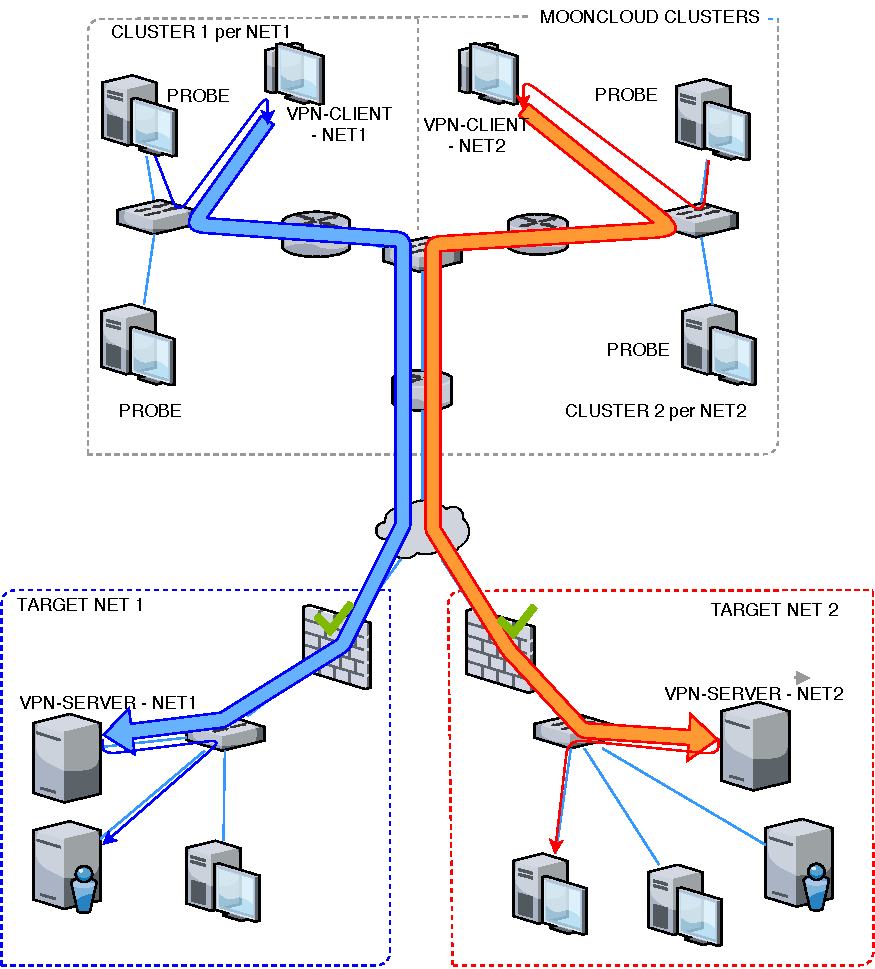
\includegraphics[scale=0.55]{img/rssc}
	\label{fig:rsmc}
	\caption[Configurazione \textit{RSSC -- Remote Server Single Client}]{Configurazione
		\textit{RSSC -- Remote Server Single Client}. Per ogni cluster dedicato ad una certa rete target
		vi è una host che svolge il ruolo di VPN client. E' ancora richiesto che i firewall
	consentano il traffico.}
\end{figure}

Già in questa fase iniziale di studio si era previsto l'utilizzo del \textit{NAT al contrario},
un termine coniato qui per indicare un particolare utilizzo del NAT. 
Si supponga di realizzare una VPN tra due reti $A$ e $B$, e che
nella rete $B$ non si possano modificare rotte. Si definisce $VPN\_A$ il dispositivo
VPN nella rete $A$ (non
importa se sia client e server), ed allo stesso modo si definisce la sua controparte $VPN\_B$.
I pacchetti ricevuti da $VPN\_B$ provenienti da $VPN\_A$ hanno come indirizzo IP uno appartenente
ad $A$, e sono immessi in $B$ senza modifiche. Le risposte a tali pacchetti dovrebbero essere inoltrate
a $VPN\_B$, ma poiché non si è configurata nessuna rotta perché non è stato possibile, saranno invece
inoltrate al default gateway di $B$.

Il \textit{NAT al contrario} consiste nell'applicare la traduzione degli indirizzi su $VPN\_B$
ai pacchetti che provengono dalla VPN, in modo da immetterli in $B$ con l'indirizzo IP
sorgente uguale a quello di $VPN\_B$. Le risposte a tali pacchetti modificati giungono 
senza problemi a $VPN\_B$, perché hanno come destinazione un IP della stessa rete, per cui non
si contatta il default gateway.
% Si supponga di
% essere nella situazione delle due reti elencate precedentemente, ma in cui non vi sia
% possibilità di intervenire sulle rotte nella rete $A$ (non si sono ancora viste quali rotte,
% ma si è detto che sono necessarie delle rotte introdotte sull'intera rete) perché essa è
% la rete target, e quindi si vogliono limitare gli interventi in essa.
% I pacchetti inoltrati da $s$ (nella rete $A$) verso la rete e provenienti da $B$, hanno
% come indirizzo IP sorgente un indirizzo IP in $B$. Una volta che tali pacchetti
% sono stati ricevuti da un host di $A$, esso non ha modo di sapere che le risposte devono
% tornare ad $s$ (proprio perché non vi sono rotte configurate), e quindi invierebbe il
% pacchetto al proprio default gateway, che quindi lo dropperebbe (trattandosi di una
% destinazione con indirizzo IP privato).\\
% Il \textit{NAT al contrario} consiste nell'applicare NAT sui pacchetti
% da $s$ (o da $c$ a seconda se sia client o server nella rete target) provenienti dalla
% VPN e destinati alla propria rete: in questo modo raggiungono l'host target con l'indirizzo IP
% di $s$, che si trova nella stessa rete del target, e per tale ragione il target può
% inviare ad $s$ le risposte senza passare dal default gateway.\\
Questo meccanismo è stato descritto in maniere molto sintetica, e poiché è una soluzione che è stata
davvero applicata, viene analizzato molto più nel dettaglio nel capitolo dedicato alle configurazioni
di OpenVPN.

Tra queste topologie, si anticipa che quella scelta è \textit{LS}.


% \section{Motivazioni}
% TODO.

\section{Introduzione alle tecnologie}

\begin{table}
	\begin{tabular}{|p{3.3cm}|p{2.7cm}|p{3.1cm}|p{1.7cm}|p{3cm}|}
		\hline
		Technology                      & Procollo di trasporto   & Protocollo incapsulato     & Passa fw. stringenti & NAT Traversal               \\
		\hline
		OpenVPN                         & TLS over TCP/UDP        & Ethernet/IP                & No                   & Sì, keepalive-based        \\
		\hline
		IPsec (IKEv2)                   & IPsec                   & IP                         & No                   & Sì                         \\
		\hline
		SoftEther                       & HTTPS (anche ICMP, DNS) & Ethernet/IP                & Sì                  & Sì, parzialmeente          \\
		\hline
		L2TP/IPsec (IKEv1)              & IPsec                   & IP                         & No                   & Sì (con SoftEther)         \\
		\hline
		\hline
		SSTP                            & HTTPS                   & PPP (IP)                   & Sì                  & Sì (con SoftEther)         \\
		\hline
		OpenConnect (Cisco Any Connect) & DTLS e HTTPS            & IP                         & Sì con HTTPS        & ?                           \\
		\hline
		OpenSSH                         & SSH                     & Ethernet/IP/TCP            & No                   & ?                           \\
		\hline
		WireGuard                       & WireGuard (UDP)         & IP                         & No                   & Sì, keepalive-based        \\
		\hline
		L2TPv3/IPsec                    & IPsec                   & Ethernet (e altri layer 2) & No                   & Sì (con IKEv2 o SoftEther) \\
		\hline
		EtherIP/IPsec                   & IPsec                   & Ethernet                   & No                   & Sì (con IKEv2 o SoftEther) \\
		\hline
		PPTP                            & GRE                     & PPP (IP and others)        & No                   & No                          \\
		\hline
	\end{tabular}
  \caption[Tecnolgie per VPN. Con ``Protocollo di trasporto'' si intende
  quale è il protocollo di più alto livello in cui si incapsulano i pacchetti indicati
  dalla colonna ``Protocollo incapsulato''. Per ``fw stringenti'' si intendono firewall
  in grado di fare filtraggio al livello applicativo.]{Principali tecnologie per VPN.}
  \label{tbl:vpn-comparison}
\end{table}

Questa sezione è demandata all'analisi delle principali tecnologie VPN. Per ciascuna
si elencano i principali passi da compiere per configurare una VPN, unitamente ad una valutazione
della migliore topologia, tenendo sempre presente che si vuole limitare il più possibile
il numero di configurazioni da effettuare nella rete target.

Una nota prima di proseguire: durante tutto questo capitolo ed il prossimo, si utilizzerà
il termine \textit{pacchetto} per indicare una generica sequenza di byte di un generico
protocollo, presente in un certo momento in un host dopo essere stata ricevuta o prima
di essere inviata, oppure in viaggio sulla rete. Sono perfettamente consapevole che per
ogni livello dello stack ISO/OSI vi sia un termine specifico per indicare tale
sequenza, ad esempio \textit{frame} per il livello 2 con Ethernet, oppure \textit{datagrammi}
per il protocollo UDP, e così via. Tuttavia, come si è visto dalla tabella \ref{tbl:vpn-comparison},
le VPN possono funzionare su diversi protocolli di trasporto (non solo al livello 4),
e possono altresì incapsulare
pacchetti di livelli divrersi. Per questa ragione ho scelto di utilizzare
\textit{indiscriminatamente} il termine \textit{pacchetto} per riferirmi ad essi.


% TODO check if I already said this
Tra le soluzioni indicate di seguito, la prima scelta è stata SoftEther. Per motivi che
verranno spiegati in seguito, la soluzione definitiva è poi OpenVPN.
